\section{Technical Specification}
\label{sec:tech}

\begin{figure}[h]
\begin{center}
\epsfig{file=archi.eps,width=0.85\columnwidth}
\caption{PredicTV System Architecture}
\shrink
\label{fig:archi}
\end{center}
\end{figure}

Figure \ref{fig:archi} illustrates the system architecture.
The core recommendation engine consists of two modules:
the offline web information extraction module and the online
recommendation module. The first module collects in advance weekly TV schedule,
identifies program titles and show times, and then extracts relevant
information about programs from web. 
The second module maintains user viewing model
dynamically and by comparing the similarity between the 
current user model and programs, 
recommends the most relevant programs to the user in real time.
We next present these two modules in greater details.

%Communication module receives users' channel switching requests,
%transfers them to Recommendation module, and outputs
%recommendations to the user. Database module stores all the program
%models and dynamically changing user viewing models. We next focus on
%the other key components: information extraction module and
%recommendation module.
%
%The Information Extraction module has two tasks. One is to crawl HTML pages  
%about TV programs from the internet, another is to extract 
%important attribute-value pairs from the pages. 
%We use Baidu and Google for the first task. 
%%For a program
%%that we want to collect its information, we form an URL based on Baidu
%%and Google's rules. Then we send HTTP requests to both these two sites
%%and get replies. Baidu and Google will reply the URLs of websites most fit
%%the key word we provide, so we send HTTP requests again and get HTML files
%%we need. Though Baidu and Google help us to search the websites most
%%related to our key words, there will still be some noise in the HTML files,
%%so we define some patterns to match information we need.
%
%Recommendation module is the core of our system. It uses users' viewing
%behaviour information as the
%input of its analysis process then replies recommendation results to users
%via Communication module. Since in mainland China, we don't have standard
%and detailed TV program information available, we have to obtain such
%information ourself. That's why Information Extraction module is involved
%in our system. It grabs HTML files from the internet, filters unnecessary
%parts, then passes them to Recommedation module. 

\subsection{Program and Viewer Model}
Before discussing the details of the two modules, we first introduce the
structure of our program and viewer model. A program model is basically a list
of attribute-value pairs. Attribute is the property of 
a program such as director, 
cast of a movie, or host of a talk show.
For certain attribute like cast of a movie, 
the value can be a set of names rather than
a single value.
In order to extract such properties or attribute values, 
we employ a statistical method.
First, we gather the list of programs, and then use 
search engine to find related pages of these programs. 
In the pages returned, we use simple but strict patterns to
match key-value pairs then choose keys which appeared more frequently 
to form an attribute list. 

A viewer model is the accumulation of program models, so the structure
is the same with program model. 
What's different is that in program model, each attribute-value
pair contains a set of values, whereas in viewer model, each value is also
is associated with a weight, which represents how important that 
value is for the owner of the model.

\subsection{Web Information Extraction}
The module first run a crawler to download TV
schedules for the coming week. As long as schedules are ready, 
before we use search engine to find out related pages for programs, 
we need to do some preprocessing on the program
name, because program names in the TV schedule may contain 
noises like type, subtitle and episode number, which affect the results
returned from search engine. After preprocessing, 
the modified program names are put on search engines like Google and Baidu. 
Ideally we will get many related
pages containing the information we need. 
As discussed in previous section, we automatically
form an attribute list for program model. 
For each attribute, we use a simple pattern to match
the context of that attribute and extract values for that attribute.

\subsection{Model Update and Recommendation}
When a viewer turns on TV, she may switch between different channels.
We capture her actions and try to predict her likes and dislikes. 
From the viewing history, we can collect the duration the viewer
views each program. We assume that the longer viewer views one program, 
the more she likes that program. 
We use this criteria to update viewer model. 
When the viewer switch to a new channel, 
a viewing record containing the old channel id, 
timestamp and duration viewer stays on that
channel is sent to server. According to channel id and timestamp, 
we find out what program viewer was previously 
watching and get the program model for viewer model updating. 
We merge program model into viewer model. 
The duration the user has spent on a program is translated into
the weight for each value in viewer model. 
All values in program model will be added to viewer model. 
If viewer model already contains that value, the weight of value will be
increased, otherwise that value is directly added to viewer model. 
We have a restriction on the size of value
set in each attribute. If the set is full, 
we remove value with the lowest weight. 

In the recommendation step, we first get a list of candidate programs to
be recommended. These are typically programs shown right now or in the near 
future. For each program in the list, we calculate the similarity 
between that program model and viewer model using Equation (\ref{eq-sim}),
and we return the top 3 programs as recommendation result. 

\begin{equation}
P_u(p) = \sum_{i=1}^nw_i\delta(v_{u_i},v_{p_i})
\label{eq-sim}
\end{equation}

$\delta(v_{u_i}, v_{p_i})$ is used to calculate the similarity between value of users and value of programs.
For each attribute in the attribute-value list, 
taking into account the different types of attributes, we design three
different implementations of function $\delta(v_{u, i}, v_{p_i})$.

For title, its value is normally a single chinese string. 
Comparing the whole string is not good enough,
therefore we use a segmentation tool to split the whole string 
into several phrases to form a set, and use Jaccord similarity here.

For time, since its value is a range, we can calculate the intersection and union of two time
range. Then divide the length of intersection by the length of union and use the ratio as the similarity.

For other attributes, the value of the attribute is also a set, so we also use Jaccord similarity, but we make some change this
time. When calculating both the intersection and union, for every value in the intersection or union, instead of
adding 1 to the size of intersection or union, we add the weight of that value. So the size here is a weighted size.

In our equation, each attribute similarity has a weight parameter $w_i$. 
Our concern is that
for different users, the effect of one attribute which influences user's choice is different. $w_i$ is
used to define the importance of one attribute to users. For each attribute, 
$w_i$ is the max value weight divided by
the sum of value weight in that attribute.
